\documentclass[UTF8]{ctexart}
\usepackage{graphics}
\usepackage{amsmath}
\usepackage{xcolor} 
\usepackage{float}
\usepackage{subfig}
\usepackage{indentfirst}
\setlength{\parindent}{2em}
\title{工作计划}

\author{冯浩哲}
\begin{document}
\section{研究问题简介}

我们本次研究的主要目的是优化医学图像分析中的数据标注流程,如\ref{fig:traditional_process},\ref{fig:improved_process}所示。\ref{fig:traditional_process}展示的是传统的医学图像分析流程,它需要医生对所有无标注的图像进行逐个标注,并利用图像及其标注训练深度学习模型。在\ref{fig:improved_process}中,我们对传统流程中的数据标注流程提出了一种改进方法,这种改进方法能基于图像本身的特征对图像进行筛选,从而找出在所有图像中最具有代表性,也就是最具有标注价值的图像进行标注。这种改进方法的好处在于可以减少医生标注的工作量,同时可以解决用于训练的图像类别不均衡的问题。

    \begin{figure}[!h]
        \centering
        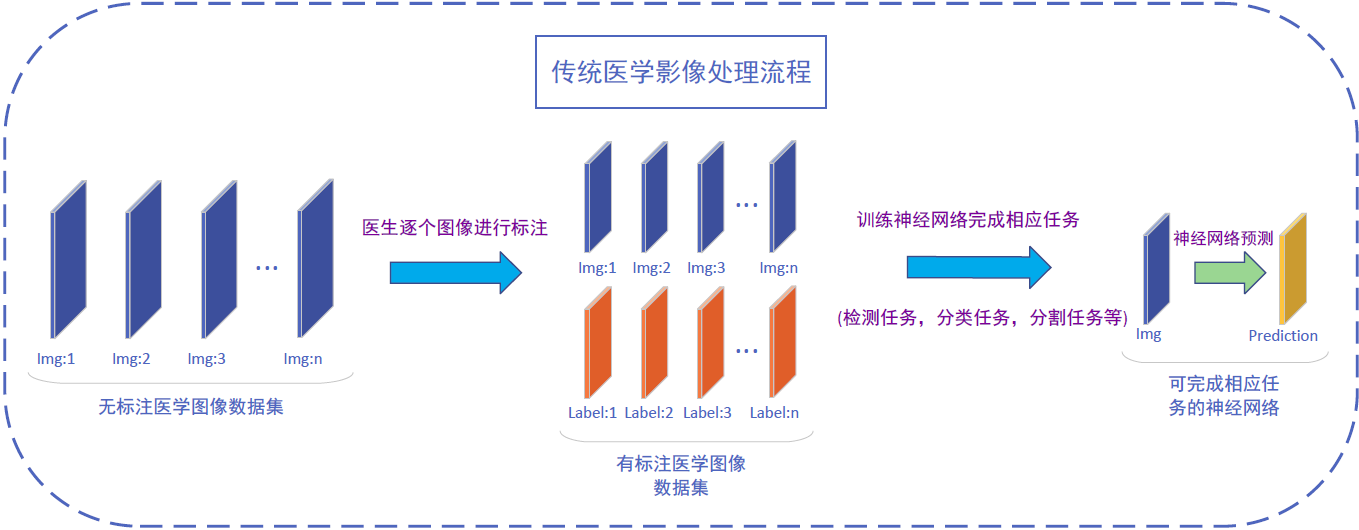
\includegraphics[width=1\linewidth]{traditional_process.png}
        %\caption{传统医学影像处理流程}%
        %\label{fig:traditional_process}%
    \end{figure}

% \begin{figure}[!h]%
%     \centering
%     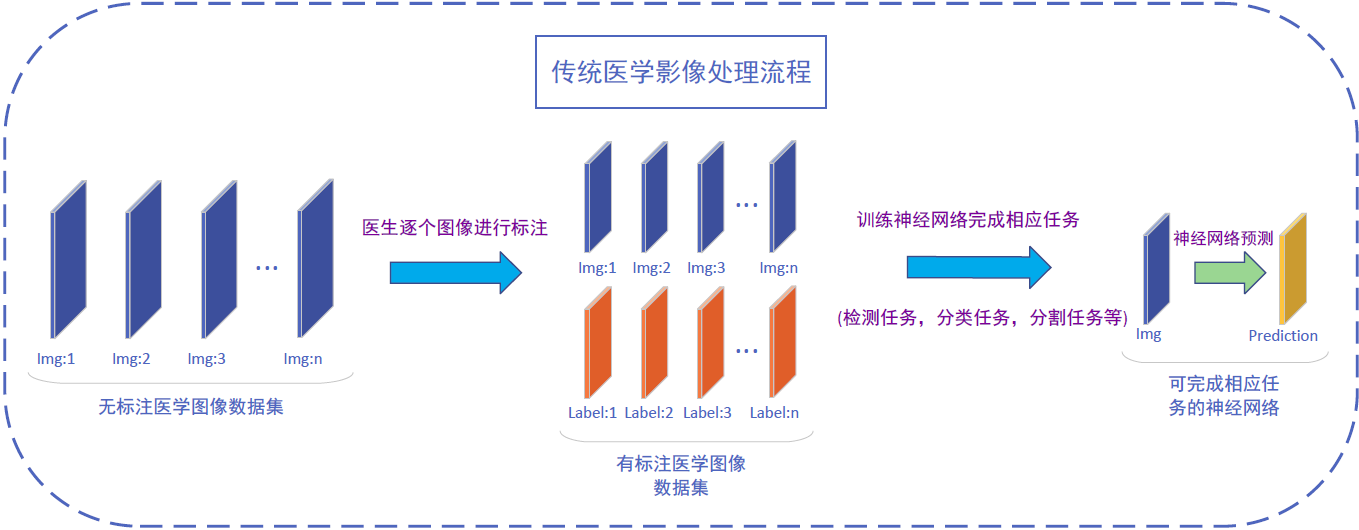
\includegraphics[width=1\linewidth]{traditional_process.png}
%     \caption{\label{fig:traditional_process}传统医学影像处理流程}
% \end{figure}

% \begin{figure}[!h]%
%     \centering
%     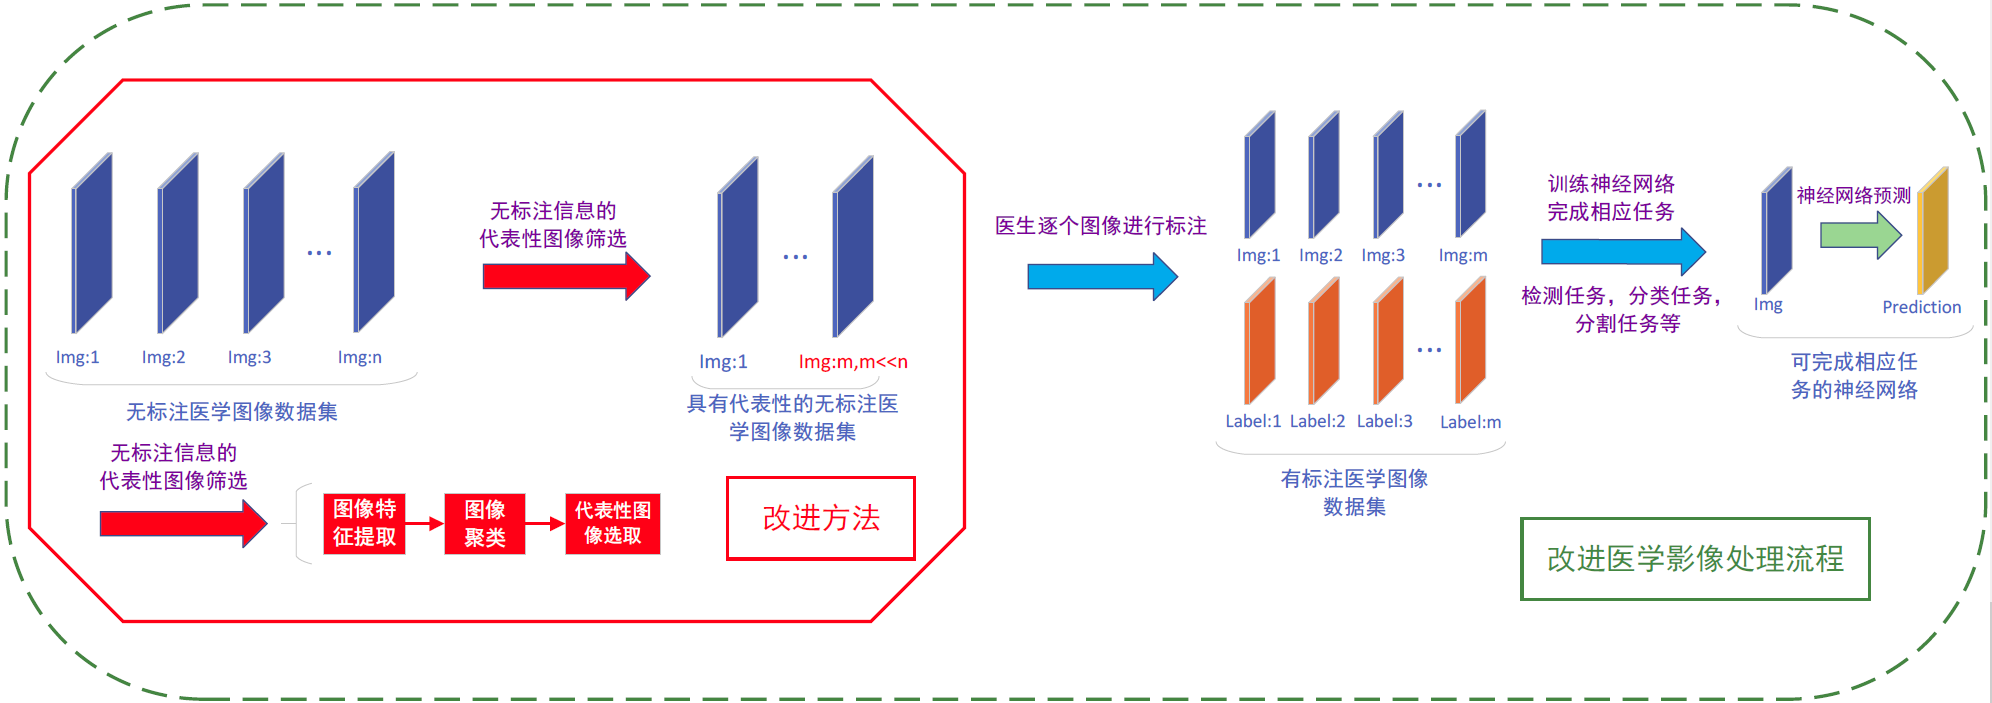
\includegraphics[width=1\linewidth]{improved_process.png}
%     \caption{\label{fig:improved_process}改进医学影像处理流程}
% \end{figure}

这项任务大部分时间是由经过专业培训的影像科医生来完成的。考虑到影像识别任务大都是机械而且目的性极强的检测与分割任务,如果能让计算机来完成此类任务,那么我们在医学诊断上的效率将大大提升,而也将极大节省医生的人力资本。
\bibliography{work_plan}
\bibliographystyle{ieeetr}
\end{document}